\section{Implementation}
This section explains how JavaGrok's toolchain works. Additionally it explains
how the exception analysis is implemented.

\subsection{Toolchain}

\begin{figure*}
\centering
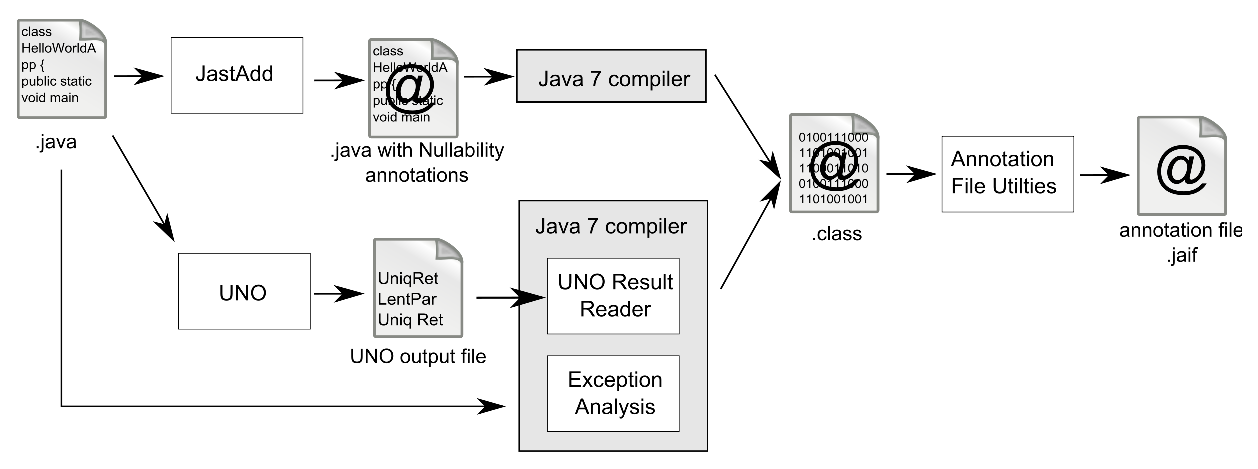
\psfig{file=figures/technicalApproach/from_source_to_jaif.eps, width=5.0in}
\caption{Toolchain from source to JAIF}
\label{fig:from_source_to_jaif}
\end{figure*}

To infer information about Java code we use two existing inference tools and 
an exception inference developed by ourselves and combine their output. 
Too aid in writing our own analyses, we have additionally developed a simple 
framework. 

To combine the results of disparate analyses we have to convert their results
into a common format.  We use the JAIF~\cite{JAIF}
(Java Annotation Index File) format for that purpose.  Some analyses provide 
annotated bytecodes which can be easily extracted into JAIF format, and 
others provide textual results for which we will read the results into our framework.

Figure~\ref{fig:from_source_to_jaif} 
illustrates the stages from the source to JAIF in our toolchain, explained 
below. While figure~\ref{fig:from_jaif_to_javadoc} shows how JavaGrok
puts the annotations back into the source files and generates the HTML
documentation.

\begin{figure*}
\centering
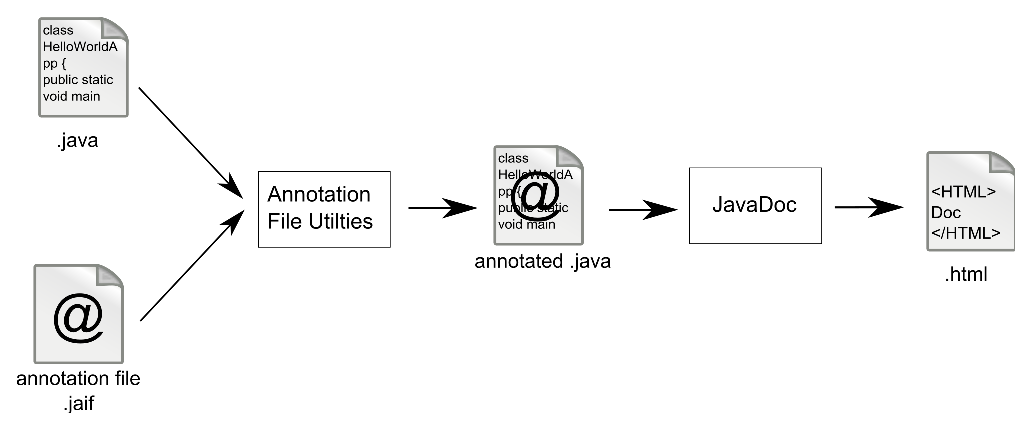
\psfig{file=figures/technicalApproach/from_jaif_to_javadoc.eps, width=5.0in}
\caption{From JAIF to Javadoc}
\label{fig:from_jaif_to_javadoc}
\end{figure*}

In a first step JavaGrok invokes Uno to process the source code to annotate. 
Uno stores its inferred properties in a single separate file. We changed Uno's 
output format slightly to make it easier to parse it automatically.
During the compilation process the Java 7 compiler reads in Uno's results 
to add annotations at the correct places. 
At the end of this compilation the class files contain retention and uniqueness
annotations. These then get extracted into files in the JAIF format with the
help of the annotations file utilities AFU~\cite{AFU}.

Analog to the capturing and leaking annotations the 
The exception analysis is part of the Java 7 compiler too. Analogously to the

JastAdd processes the source code and adds nullability annotations
directly into the source code. After that the source code with annotations
is compiled to class files which contain the annotations which  
get extracted using the annotation file utilities.

Once the results of the various analyses have been collected into a set of
annotation files, the annotation file utilities merge
those annotations back into the original source. The annotated source
code is now one of JavaGrok's output formats. Additionally Javadoc processes
the annotated source and combines the newly added annotations into the html
documentation.

\subsection{Exception analysis}
\label{sec:exception_analysis}
TODO: Colin's text here